\documentclass[conference]{IEEEtran}

% to enable \thanks
\IEEEoverridecommandlockouts

\usepackage{cite}
\usepackage{graphicx}
\usepackage{color}
\newcommand{\unit}[1]{\ensuremath{\, \mathrm{#1}}}

\graphicspath{{plots/}}

\begin{document}

\title{Efficient Extraction of Regional Subsets from Massive Climate Datasets
using Parallel IO}

\author{
\IEEEauthorblockN{
    Jeff Daily\IEEEauthorrefmark{1},
    Karen Schuchardt\IEEEauthorrefmark{1} and
    Bruce Palmer\IEEEauthorrefmark{1}
}
\IEEEauthorblockA{
    \IEEEauthorrefmark{1}
    Pacific Northwest National Laboratory\\
    jeff.daily,karen.schuchardt,bruce.palmer@pnl.gov
}
\thanks{TODO Wei-keng Liao}
}

\maketitle

% For peer review papers, you can put extra information on the cover
% page as needed:
% \ifCLASSOPTIONpeerreview
% \begin{center} \bfseries EDICS Category: 3-BBND \end{center}
% \fi
%
% For peerreview papers, this IEEEtran command inserts a page break and
% creates the second title.  It will be ignored for other modes.
\IEEEpeerreviewmaketitle

\begin{abstract}
\label{section:abstract}

The size of datasets produced by current climate models is increasing rapidly
to the scale of petabytes.  To handle data at this scale parallel analysis
tools are required, however the majority of climate analysis software is
serial and remains at the scale of workstations.  Further, many climate
analysis tools are designed to process regularly gridded data but lack
sufficient features to handle unstructured grids.  This paper presents a
data-parallel subsetter capable of correctly handling unstructured grids while
scaling to over 2000 cores.  The approach is based on the partitioned global
address space (PGAS) parallel programming model and one-sided communication.
The paper demonstrates that parallel analysis of climate data succeeds in
practice, although IO remains the single greatest bottleneck.

\end{abstract}

\section{Introduction}
\label{section:introduction}

\cite{TEST:TEST}TODO

In this paper, we present...

Fincally, section \ref{section:conclusion} presents our conclusions.

\section{Requirements}
\label{section:requirements}

The requirements for our software stem from the growing need for parallel
analysis in the domain of climate science\cite{MODSIM07:LOT} but also from
the use of the geodesic grid.

\subsection{Geodesic Grid}
\label{subsection:grid}

Until recently, climate and weather models have primarily been simulated on
structured grids that divide the latitude and longitude axes in even
increments, resulting in logically structured simulation grids.  Standard
conventions for describing this data in the NetCDF data model have been
formalized by the Climate and Forecast (CF) conventions\cite{CF}.  CF defines
conventions and metadata standards that enable both human and computer
interpretation of the data.  Human interpretation is supported through the use
of standard names while the definition of spatial and temporal properties of the
data have enabled an extensive set of tools for data manipulation and display
such as \cite{NCO}, \cite{OPeNDAP}, and \cite{FERRET}.  The CF Conventions
have been evolving to support many variations of structured grids including
Orthographic, Polar stereographic, Transverse Mercator, and many others. 

The GCRM uses a geodesic grid.  The geodesic grid is created by recursively
bisecting an icosahedron of 20 triangular faces and twelve vertices and
projecting the resulting faces onto a unit sphere.  These vertices
represent the centers of hexagonal grid cells with the exception of twelve
pentagons (the centers of the original twelve vertices.) See Fig.
\ref{fig:geodesic} for an example of the first stage of bisection and
projection, followed by the definition of one of the hexagons.  Once the
desired grid resolution is reached (Fig. \ref{fig:panels}(left)), the
original triangles of the icosahedron are paired such that each pair shares an
edge. The grid points generated from each pair form a logically
structured block (Fig. \ref{fig:panels}(right)) that can be stored
as a set of regular square arrays of data points.  Further details can be
found in \cite{GEODESIC}.

\begin{figure}[!t]
\center
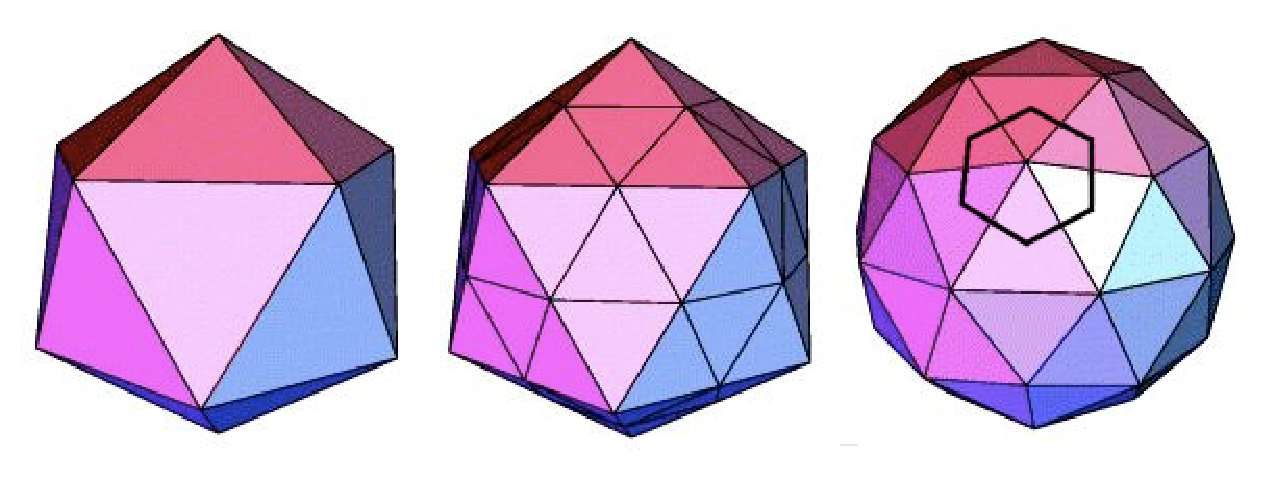
\includegraphics[width=3.5in]{images/geodesic2}
\caption{The geodesic grid is created by recursively bisecting an icosahedron
of 20 triangular faces and 12 vertices and projecting the resulting faces on
to a unit sphere.  The first recursion and a sample hexagonal cell can be seen
here.}
\label{fig:geodesic}
\end{figure}

\begin{figure}[!t]
\center
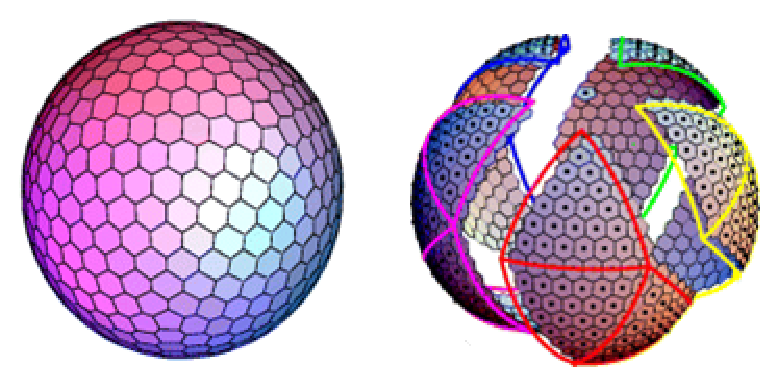
\includegraphics[width=2.5in]{images/panels}
\caption{Once the desired grid resolution is reached (left), if the original
triangles of the icosahedron are paired such that each pair shares an edge,
then the grid points generated from each pair form a logically structured
block (right).  These blocks can be stored as a set of regular square arrays
of data points.}
\label{fig:panels}
\end{figure}

From the previous description, it can be seen that the geodesic grid used by
the GCRM is fairly regular.  However, the horizontal dimension has some
important properties in common with unstructured grids: the grid coordinates
are not monotonic and simple conventions are not available for identifying the
neighbors of all cells.  As a consequence, it is necessary to provide more
information about the topology of the grid.  Other unstructured grids such as
triangular, cubed sphere \cite{CUBE}, and arbitrary unstructured polygons are
also being applied to various models.  There is a recognized need to extend
the CF conventions to unstructured grids so that general data analysis,
regridding, and display tools can be developed.  As yet, no such standard
exists.  Lacking a standard, development of general purpose tools has been
slowed.  However some preliminary tools and approaches have progressed by
focusing on the in-memory operations and abstracting the data loading from the
processing \cite{UGRID}. 

Although the geodesic grid is fairly structured, we choose to represent it in
an unstructured way.  Each of the grid's cells, corners, and edges are
uniquely indexed from zero.  For a given positive integer $R$, there are $N =
10 \times 2^{2R} + 2$ cells, $C = (N-2) \times 2$ corners, and $E = (N-2)
\times 3$ edges.  Increasing the value of $R$ increases the resolution of the
model.  For example, a value of $R=10$ is approximately 8 kilometers while
$R=11$ is approximately 4 kilometers.  The number of cells, corners, and edges
are represented as dimensions within a NetCDF file.

The data for the GCRM is ordered using a space-filling curve.  As seen in Fig.
\ref{fig:panels}, the data is divided into square panels.  The data within
each panel can be reorganized using a Morton-ordering scheme (also referred to
as Z-ordering).  This has the advantage that it is much easier to guarantee
that each read or write represents a contiguous chunk in the file.  The
Morton-ordering scheme works very well for square arrays that are an integral
power of 2 in dimension and is illustrated schematically in Fig.
\ref{fig:morton}.  Each array element is indexed by successive locations in
the self-similar space-filling curve.  Fig. \ref{fig:morton} shows a panel
that has been divided up into 16 blocks.  Note, however, that if the panel had
been divided into only 4 blocks, the points within each block would still lie
along a continuous segment of the space-filling curve.

\begin{figure}[!t]
\center
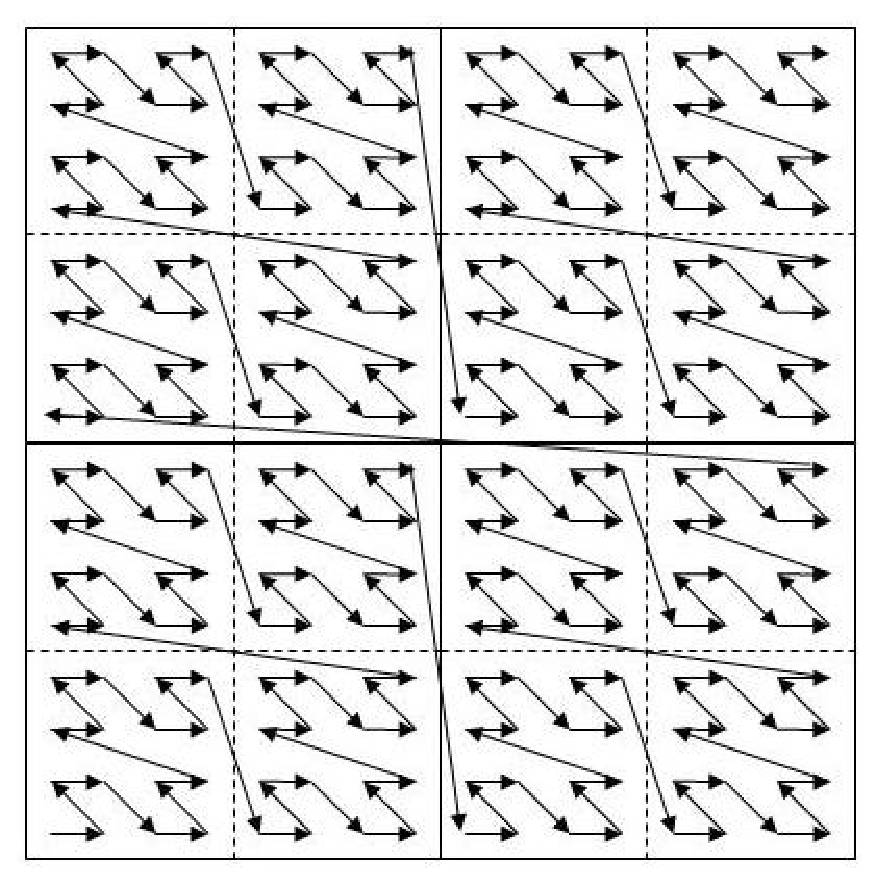
\includegraphics[width=3.5in]{images/morton}
\caption{Illustration of Morton-ordering curve for a 16x16 array of points.
Each array element is indexed by successive locations in the self-similar
space-filling curve.}
\label{fig:morton}
\end{figure}

The horizontal topology describes the connectivity relationships between
cells, nodes, and edges, all of which may have associated 3D data.  The
topology consists of three primary arrays: a mapping between cells and cell
corners, a mapping between cells and cell edges, and a mapping between edges
and corners.  Because neighbor lists are important for visualization programs
but difficult to generate in the general case, they are included as part of
the topology as the \verb+cell_neighbors(cells,neighbors=6)+ variable.  The
full list of topology variables include:

\begin{itemize}
\item \verb+cell_neighbors(cells,neighbors=6)+,
\item \verb+cell_corners(cells,cellcorners=6)+,
\item \verb+cell_edges(cells,celledges=6)+, and
\item \verb+edge_corners(edges,edgecorners=2)+
\end{itemize}

The vast majority of cells are hexagons which is why most of the last
dimensions are of size six except for the obvious case of \verb+edgecorners+.
For the twelve pentagons, the sixth value in these arrays are repeated but
could just have easily been set to a negative index and interpreted
appropriately.

The horizontal geometry describes the longitude and latitude location of each
object.  That is, there is one latitude and one longitude array for each of
the topology objects (cell centers, corners, and edges).

The vertical grid consists of layers sandwiched between interfaces with the
number of layers equal to the number of interfaces minus 1.   Because grid
variables are associated with both locations, layers and interfaces are
defined as dimensions.  They can be thought of as two distinct vertical grids
from a representation standpoint.

The data model is designed to support efficient model output, fully describe
the grid topology, and provide sufficient information for tessellation to
triangles for 3D visualization.  The approach taken with the model is to adopt
the CF conventions to the extent possible and adopt early ideas circulating
within the community.  However, as many of the details have not been decided,
custom data analysis tools are currently required and further modifications to
the tools may be needed to conform to evolving standards.

\subsection{Data Parallelism}

Larson, Ong, and Tokarz note that the current popular climate data analysis
packages remain single-processor applications. These lack the memory required
to handle large data volumes as well as the processing power to analyze the
data in a timely fashion\cite{MODSIM07:LOT}.  Although they emphasize using
OpenMP as a first step toward parallelism, we instead emphasize using a
distributed data model first.  Well designed communication libraries such as
the Message Passing Interface (MPI)\cite{MPI} may already take advantage of
shared-memory parallelism within a compute node or multi-core desktop
computer.

The data parallelism offered by libraries such as MPI or Global Arrays is
absolutely necessary to handle the size of data of modern climate models.  An
edge data variable of the geodesic grid at an approximate resolution of 4
kilometers and 100 levels is nearly $10 \times 2^{2 \times R} \times 3 \times
100 \times 4 \unit{bytes} \approx 50 \unit{gigabytes}$ in size, where $R=11$.
Even a modest number of these variables will surpass the memory available in
most desktop systems and even some small clusters.

\subsection{Fast IO}

For data of this size, efficiently reading from and writing to disk requires
the use of parallel IO libraries such as Parallel-NetCDF\cite{PNETCDF} or
HDF5/NetCDF4\cite{HDF5}\cite{NETCDF}, both of which are in turn built on top
of the MPI-IO libraries\cite{MPIIO}.  Currently, GCRM output is stored in
netCDF\cite{NETCDF} files, a format for storing array-oriented
machine-independent data.

\subsection{64bit Libraries}

64bit libraries are also required for the GCRM output at 4 kilometer
resolution.  At this resolution, the GCRM output already requires 64bit file
offsets.  At resolutions smaller than 4 kilometers, the GCRM output will begin
to produce edge variables that exceed the 4 byte limit for array indexing.

\subsection{Dataset Abstraction}

Model output is often distributed across many files for a given model run.
There are any number of schemes for organizing so many files, e.g. one variable
per file with multiple timesteps per file, separating out the grid into a
separate file, one timestep per file with multiple variables.  The
reconstitution of these files into a logical set of variables and metadata is
an established practice\cite{NcML,THREDDS}.  We emphasize that the aggregation
of files into an abstract dataset is required in order to operate on the data
itself.  Operations on a dataset are more intuitive than needing to know the
addling details of which files hold which variables.

\subsection{Maintenance of Topology Variables}

Regular grids such as the Cartesian, rectilinear, or curvilinear grids lend
themselves to representations as multidimensional arrays such that logically
adjacent cells are either adjacent in memory or can be located via a
shape-based index calculation.  Although some attempt is made to keep
logically adjacent cells nearby in memory, geodesic grids do not have the
luxury of using relatively simple shape-based index arithmetic to locate
neighbors.

The topology variables mentioned in Section \ref{subsection:grid} are not
unique to our grid; any grid could be described using a similar set of
variables.  However, since topology is often implicitly defined for other
grids, these variables are not correctly handled by current software.  When a
subset occurs, the indices of these variables must be updated to reflect the
remaining corners, edges, and cells as seen in Fig. \ref{fig:subset}.

\begin{figure}[!t]
\center
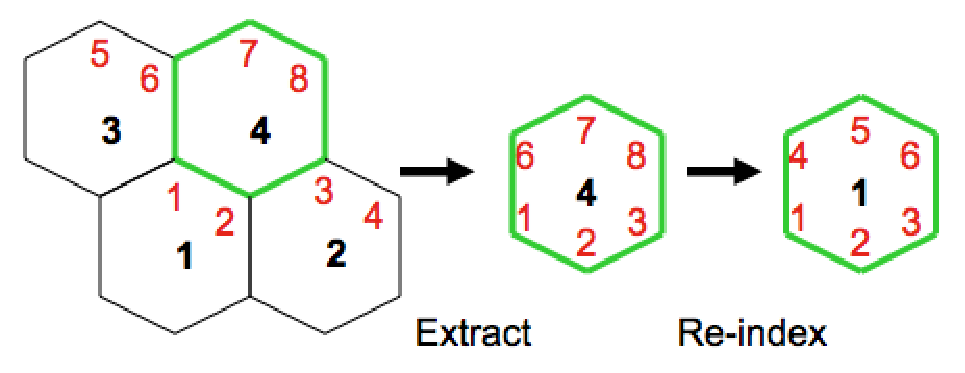
\includegraphics[width=3.5in]{images/Subset1}
\caption{Maintenance of Topology Variables and Integrity of Entire Grid Cells.
The hexagonal cells remain well-formed during extraction while the indices of
the corners are reindexed to reflect the fewer overall corners in the subset.}
\label{fig:subset}
\end{figure}

\subsection{Maintaining Integrity of Entire Grid Cells}

Howe and Maier detail the properties of well-formed grids in \cite{UGRID}.
Proper subsets should maintain the same well-formed properties of the original
in order to remain useful to further analysis.  Therefore, the cell and its
surrounding corners and edges must remain intact during a subset as seen in
Fig. \ref{fig:subset}. The first step in forming a subset results in a
collection of cell and corner indices that do not form a contiguous sequence
of integers. The cells and corners must be reindexed the corresponding topology
lists updated to give a well formed description of the topology.

\section{Design}
\label{section:design}

In this section we describe the design of our classes and algorithms based on
the requirements established in Section \ref{section:requirements}.

\subsection{Subsetter User Interface}

The subsetter is the first in a series of planned parallel command-line tools
based on unstructured grids, the PGAS model, and one-sided communication.  It
takes arguments indicating specific variables (-v), dimension ranges (-d) to
extract, or a latitude and longitude bounding box (-b).  Parallel climate
analysis tools require the use of common startup programs (such as "mpirun" or
"mpiexec" for MPI programs) capable of spawning parallel jobs on a cluster of
other parallel architecture.  Users of these tools must become familiar with
how to run parallel software.  Looking past the particular use of "mpiexec
-np" below to invoke our MPI program with a given number of processors,
example usage of the subsetter looks like:

\begin{itemize}
\item mpiexec -np 128 subsetter -b 20,-20,160,90 -v vorticity january.nc february.nc MJO\_vorticity\_janfeb.nc
\item mpiexec -np 64 subsetter -b 90,0,180,-180 -d levels,1,5 geopotential.nc out.nc
\end{itemize}

Similarly, the NetCDF Operator's \emph{ncks} application\cite{NCO} is run
like the following, noting that \emph{ncks} does not aggregate input files:

\begin{itemize}
\item ncks -X 90,160,-20,20 -v vorticity january.nc MJO\_vorticity\_january.nc
\item ncks -X -180,180,0,90 -d levels,1,5 geopotential.nc out.nc
\end{itemize}

\subsection{Dataset Abstraction}

A dataset abstraction is essential for the comprehension of these large
datasets, hiding the details of which files contain which data.  The subsetter
currently supports two forms of input file aggregation, either across a
specified dimension e.g. time or by taking the union of all input files such
that duplicate dimensions and grid and topology variables within later files
are ignored.  These forms of aggregation are modeled after what is available
when using NetCDF Markup Language\cite{NcML}.  NcML input is not directly
supported at this time but is planned for a future release. 

\subsection{Parallel IO Abstraction}

IO operations are hidden behind abstract base classes.  Any IO library can be
supported so long as the data structures conform to the Common Data Model
(CDM)\cite{CDM}.  This is similar to how the Java NetCDF library works,
supporting many different data formats conforming to the CDM\cite{JavaNetCDF}.
Further, differing IO strategies using the same IO library can also be
developed behind the same API.  The use of Parallel-NetCDF was selected
because of the ubiquity of the NetCDF libraries and data format in climate
applications.

\subsection{The Global Arrays Library}

The PGAS programming model assumes a global address space which is partitioned
such that each process is associated with a local portion of the space.
One-sided communication allows a process to access another process's address
space without any explicit participation by the latter process.  Such
communication can reduce synchronization and can simplify programming.  The
Global Arrays (GA) library supports both global address spaces and onesided
communication.

The subsetter was built using the GA library for the wealth of features it
provides which are tailored to our problem domain.  GA provides a distributed
dense multidimensional array programming abstraction and the data we will be
operating over is stored as dense arrays within NetCDF files.  It should be
noted that dense distributed arrays would also work well for regularly gridded
data.  However, due to the use of unstructured grid data, the algorithm for
subsetting the data will look quite different than for the structured case.
Recall that for unstructured grids, logically adjacent cells are not
necessarily adjacent in memory.  In order to evenly distribute a subset, a
single process will need to send a varying amount of data to any number of
other processes.  Certainly a collective operation could be considered, but GA
provides the necessary functionality without needing any explicit cooperation
from any other process.  Any given process will simply put the section of the
subset into the remote process's memory which owns the subset.

There are certain GA one-sided operations which are tailored for use on
one-dimensional arrays which are used within our program.  These operations
include:

\begin{itemize}
\item \verb=GA_Patch_enum=,
\item \verb=GA_Scan_add=, and
\item \verb=GA_Unpack=
\end{itemize}

Those operations have been demonstrated in the computation of sparse matrix
multiplication\cite{GA} but are equally useful in the manipulation of
unstructured grids.  The remaining GA operations are N-dimensional and
include:

\begin{itemize}
\item \verb=NGA_Scatter=,
\item \verb=NGA_Gather=,
\item \verb=NGA_Put=, and
\item \verb=NGA_Get=
\end{itemize}

Those operations are useful for redistributing the subset data and for
querying the values of the various distributed arrays without regard to which
process owns the data being queried.

\subsection{The Algorithms}

The one-sided communication and PGAS model supported by GA allowed us to
develop some novel algorithms for the manipulation of unstructured grids.  In
this section we diagram and describe the algorithms we developed.  The vast
majority of functionality within the subsetter is provided by either
Parallel-NetCDF or GA.  GA allocates and evenly distributes the arrays.  The
starting and ending indices owned by each process are used directly to fill
the arrays using Parallel-NetCDF.  GA operations are then used to prepare the
data for packing, at which point a custom n-dimensional packing routine is
used.  After packing, evenly-distributed data is written back to disk using
Parallel-NetCDF.  (Note that instead of immediately writing the data back to
disk, any number of other mathematical operations could take place.) Of these
algorithms, the novel ones include reindexing the masks, reindexing the
topology variables, and the n-dimensional pack routine.

Each dimension of the data has two arrays associated with it, an integer array
representing a bitmask and an integer array representing the new indices of
the dimension in case of a subset.  For instance, if any of the bits are zero
(off), the corresponding indices of the index array will have negative values.
The remaining values of the index array will increase monotonically, skipping
the negative or masked indices.  The bitmasks are generated based on a
rectangular latitude and longitude region specified on the command-line, or by
specifying one or more indices of a dimension to select.  Although a
rectangular region is currently used for simplicity, once translated the
bitmasks allow for arbitrary subsets to be defined.  These bitmasks are then
used to evenly distribute the resultant subset across all processes.  Note
that these bitmask and associated index arrays are one-dimensional and
distributed.

\subsubsection{Partial Sum}

%\begin{figure}[!t]
%\center
%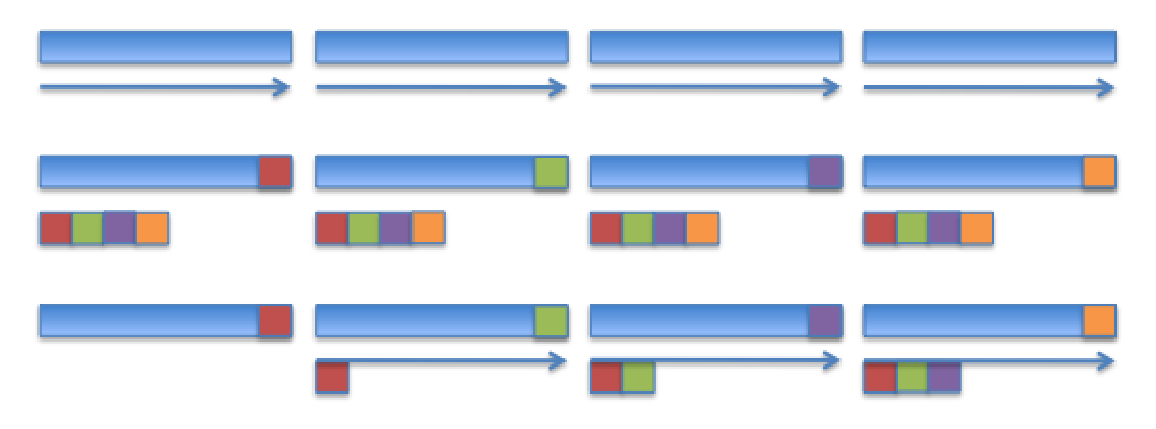
\includegraphics[width=3.5in]{images/partialsum}
%\caption{A distributed partial sum over a 1-D array.  A partial sum is first
%computed over the local portions (A), the last values of each portion are
%collected on each process (B), and lastly each local portion adds the last
%values taken from each previous process (C).}
%\label{fig:partialsum}
%\end{figure}

A partial sum of the index array associated with each dimension is useful for
later determining which process is to receive which portion of the subset
data.  That feature will be explained in more detail in Section
\ref{section:alg_pack}.  The partial sum operation here is semantically
similar to the one found in the C++ STL\cite{CXXSTL}.  It computes a series of
sums over an array from the first element through the \emph{i}th element and
stores the result of each such sum in the \emph{i}th element of a destination
array.  For example, if $x$ represents an element in the array and $y$
represents an element in the destination array, the $y$s can be calculated as:

\begin{equation}
\begin{split}
y_0 &= x_0\\
y_1 &= x_0 + x_1\\
y_2 &= x_0 + x_1 + x_2\\
y_3 &= x_0 + x_1 + x_2 + x_3\\
\ldots
\end{split}
\end{equation}

%The partial sum is computed by first performing partial sums of each local
%portion of the source array.  This operation is represented by Fig.
%\ref{fig:partialsum}A.  The last value of each local sum is then collectively
%distributed to each process as seen in Fig. \ref{fig:partialsum}B.  Fig.
%\ref{fig:partialsum}C is the last step where each local portion adds the last
%values of each process's sum which come before.

The partial sum is elegantly computed using a single call to the
\verb+GA_Scan_add+ routine.

\subsubsection{Reindexing of Dimension Index}

Creating the index array associated with a mask requires three specific GA
operations, \verb=GA_Fill=, \verb=GA_Patch_enum= and \verb=GA_Unpack=.  The
mask array is represented in Fig. \ref{fig:unpack}A with the masked bits
indicated in black.  \verb=GA_Fill= fills the index array, the array in Fig.
\ref{fig:unpack}B, with a value of $-1$.  Each process counts how many masked
bits they own and then collectively sums their count.  A third array is
created (Fig. \ref{fig:unpack}C) based on this count.  \verb=GA_Patch_enum=
enumerates the values in the newly created array starting from zero with an
increment of 1 (indicated by the arrows in Fig. \ref{fig:unpack}C).
\verb=GA_Unpack= expands the enumerated array values into the filled array
based on the associated mask array as seen in Fig. \ref{fig:unpack}D.

\begin{figure}[!t]
\center
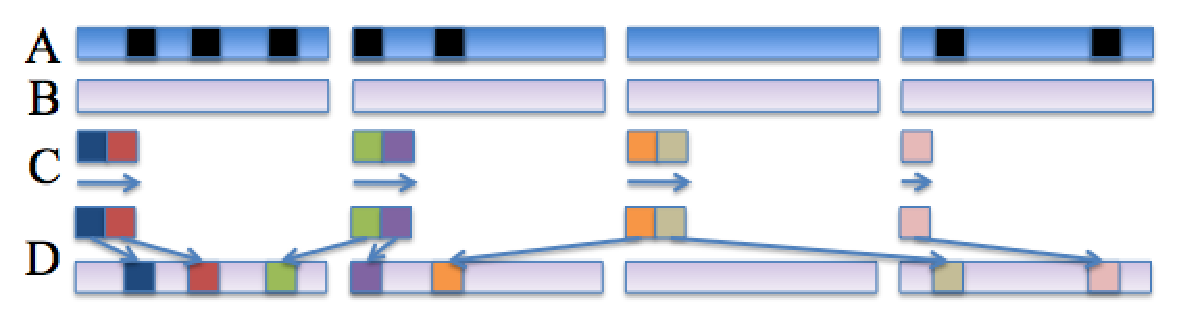
\includegraphics[width=3.5in]{images/unpack}
\caption{Reindexing of a Dimension Index.  The index array (B) is filled with
a value of $-1$.  The masked bits of (A) are tallied such that a new array (C)
is created based on the tallied size.  The new array C is enumerated and then
unpacked into the index array (D).}
\label{fig:unpack}
\end{figure}

\subsubsection{Reindexing of Topology Variables}

Recall that the topology variables are those which map from one index to one
or more other indices such as from a cell index to each of its corner indices.
A typical subset operation reduces the number of cells, corners, and edges
within the grid, so it is important to maintain the integrity of these mapping
arrays such that they map to real indices.

The reindexing of the topology variables relies on the recalculated index
array of the associated domain.  For example, when reindexing the mapping from
edges to corners, the recalculated corners index array is required (Fig.
\ref{fig:reindex}A).  The mapping values represent indices into the
recalculated index array.  The original mapping arrays are iterated over to
prepare the required indices for the subsequent GA routine \verb=NGA_Gather=
to query.  The \verb=NGA_Gather= routine gathers array elements from a global
array into a local array by specifying the desired indices.  In this way each
process gathers the new values for the mapping from the index array and then
appropriately replaces the old mapping values.  For clarity, Fig.
\ref{fig:reindex}B shows four processes gathering and replacing only the
non-negative indices, but it should be noted that all indices are replaced by
this operation.

\begin{figure}[!t]
\center
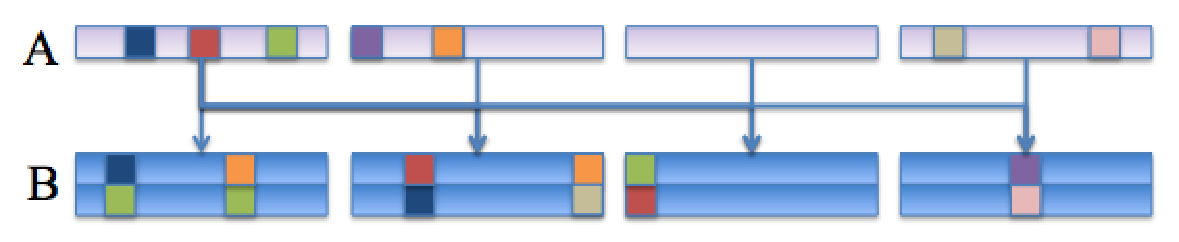
\includegraphics[width=3.5in]{images/reindex2}
\caption{Reindexing of Topology Variables.  The recalculated index array from
the Fig. \ref{fig:unpack} reindexing operation, seen here as (A), will replace
values found within the topology array (B).  Each process gathers values from
the index array after using the original values from (B) in an NGA\_Gather
call.  All values from the original index array are replaced (only replacement
of non-negative indices is shown for clarity).}
\label{fig:reindex}
\end{figure}

\subsubsection{N-Dimensional Pack}
\label{section:alg_pack}

The goal of the pack routine is to start with an evenly distributed source
array, subset it, and evenly distribute the subset.  The subset is specified
using mask arrays, one for each dimension of the source array (the blue arrays
in Fig. \ref{fig:pack} with masked bits indicated in black).  The size of the
subset is determined by counting the number of masked bits per dimension.
Each process determines where to \verb=NGA_Put()= its portion of the subset by
examining the partial sum array (the olive arrays in Fig. \ref{fig:pack}).
The values indicated in orange in Fig. \ref{fig:pack} represent the values of
partial sum array at those particular indices and are used by each process to
know where to put their portion of the subset data into the subset array.  For
example, process 1 in Fig. \ref{fig:pack} calls \verb=NGA_Put()= to place its
data starting at index (3,0).

\begin{figure}[!t]
\center
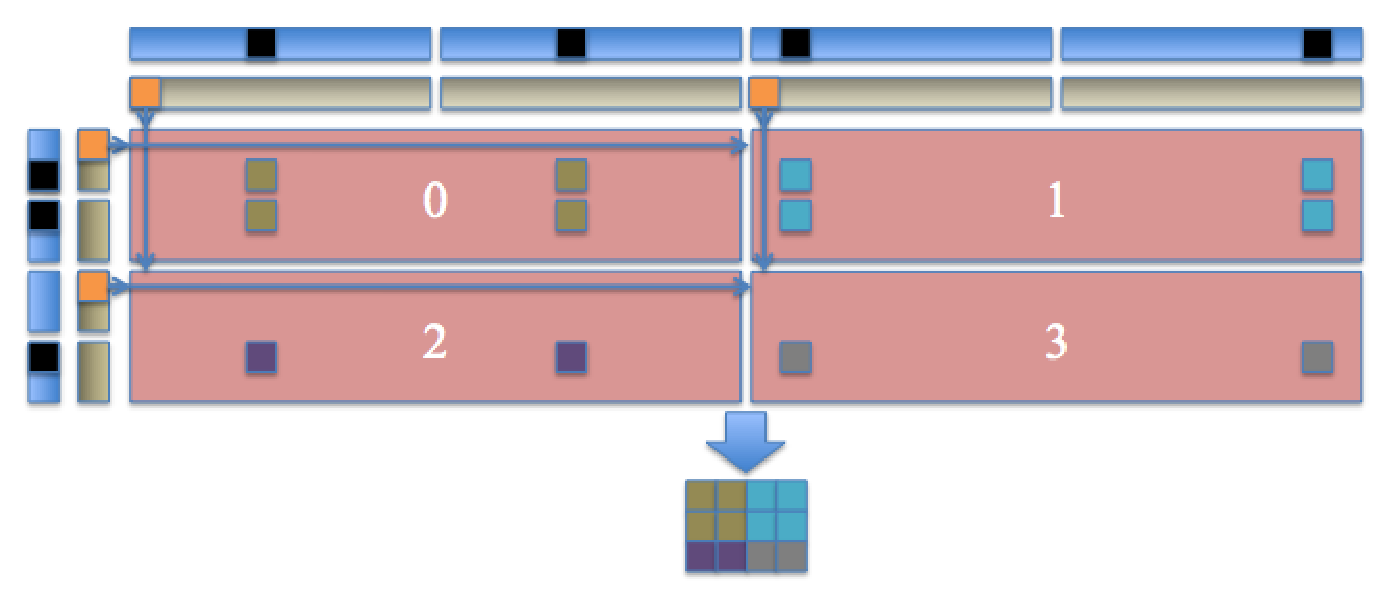
\includegraphics[width=3.5in]{images/pack}
\caption{Pack.  The blue arrays represent the masks with masked bits indicated
in black.  The olive arrays are the partial sums over the masks.  The orange
values represent the values of the partial sum array at those indices.  Each
process queries the partial sum arrays for where to put their subset data,
packs their local data based on the mask bits, and calls NGA\_Put to deliver
the subset data.  The destination array is by default evenly distributed.}
\label{fig:pack}
\end{figure}

The data location abstraction offered by GA is even more important as
differing numbers of processors and/or different data distributions are used.
As can be seen in the case diagrammed in Fig. \ref{fig:pack}, the partial sum
arrays are as evenly distributed as the data arrays.  Although GA evenly
distributes arrays by default, different distributions can be specified.  For
example, it might be beneficial to keep all vertical levels for a given region
local to a process.  The desired values from the partial sum arrays will
change process owners depending on how many processes are used or how the data
is distributed.  \verb+GA_Get+ and \verb+GA_Put+ abstract away that need to
track which process owns the data and simplifies the programming model.

\section{Evaluation}
\label{section:evaluation}

\begin{figure}[!t]
\center
\resizebox{3.5in}{!}{
% GNUPLOT: LaTeX picture with Postscript
\begingroup
  \makeatletter
  \providecommand\color[2][]{%
    \GenericError{(gnuplot) \space\space\space\@spaces}{%
      Package color not loaded in conjunction with
      terminal option `colourtext'%
    }{See the gnuplot documentation for explanation.%
    }{Either use 'blacktext' in gnuplot or load the package
      color.sty in LaTeX.}%
    \renewcommand\color[2][]{}%
  }%
  \providecommand\includegraphics[2][]{%
    \GenericError{(gnuplot) \space\space\space\@spaces}{%
      Package graphicx or graphics not loaded%
    }{See the gnuplot documentation for explanation.%
    }{The gnuplot epslatex terminal needs graphicx.sty or graphics.sty.}%
    \renewcommand\includegraphics[2][]{}%
  }%
  \providecommand\rotatebox[2]{#2}%
  \@ifundefined{ifGPcolor}{%
    \newif\ifGPcolor
    \GPcolortrue
  }{}%
  \@ifundefined{ifGPblacktext}{%
    \newif\ifGPblacktext
    \GPblacktexttrue
  }{}%
  % define a \g@addto@macro without @ in the name:
  \let\gplgaddtomacro\g@addto@macro
  % define empty templates for all commands taking text:
  \gdef\gplbacktext{}%
  \gdef\gplfronttext{}%
  \makeatother
  \ifGPblacktext
    % no textcolor at all
    \def\colorrgb#1{}%
    \def\colorgray#1{}%
  \else
    % gray or color?
    \ifGPcolor
      \def\colorrgb#1{\color[rgb]{#1}}%
      \def\colorgray#1{\color[gray]{#1}}%
      \expandafter\def\csname LTw\endcsname{\color{white}}%
      \expandafter\def\csname LTb\endcsname{\color{black}}%
      \expandafter\def\csname LTa\endcsname{\color{black}}%
      \expandafter\def\csname LT0\endcsname{\color[rgb]{1,0,0}}%
      \expandafter\def\csname LT1\endcsname{\color[rgb]{0,1,0}}%
      \expandafter\def\csname LT2\endcsname{\color[rgb]{0,0,1}}%
      \expandafter\def\csname LT3\endcsname{\color[rgb]{1,0,1}}%
      \expandafter\def\csname LT4\endcsname{\color[rgb]{0,1,1}}%
      \expandafter\def\csname LT5\endcsname{\color[rgb]{1,1,0}}%
      \expandafter\def\csname LT6\endcsname{\color[rgb]{0,0,0}}%
      \expandafter\def\csname LT7\endcsname{\color[rgb]{1,0.3,0}}%
      \expandafter\def\csname LT8\endcsname{\color[rgb]{0.5,0.5,0.5}}%
    \else
      % gray
      \def\colorrgb#1{\color{black}}%
      \def\colorgray#1{\color[gray]{#1}}%
      \expandafter\def\csname LTw\endcsname{\color{white}}%
      \expandafter\def\csname LTb\endcsname{\color{black}}%
      \expandafter\def\csname LTa\endcsname{\color{black}}%
      \expandafter\def\csname LT0\endcsname{\color{black}}%
      \expandafter\def\csname LT1\endcsname{\color{black}}%
      \expandafter\def\csname LT2\endcsname{\color{black}}%
      \expandafter\def\csname LT3\endcsname{\color{black}}%
      \expandafter\def\csname LT4\endcsname{\color{black}}%
      \expandafter\def\csname LT5\endcsname{\color{black}}%
      \expandafter\def\csname LT6\endcsname{\color{black}}%
      \expandafter\def\csname LT7\endcsname{\color{black}}%
      \expandafter\def\csname LT8\endcsname{\color{black}}%
    \fi
  \fi
  \setlength{\unitlength}{0.0500bp}%
  \begin{picture}(7200.00,5040.00)%
    \gplgaddtomacro\gplbacktext{%
      \csname LTb\endcsname%
      \put(1210,704){\makebox(0,0)[r]{\strut{} 0}}%
      \put(1210,1112){\makebox(0,0)[r]{\strut{} 100}}%
      \put(1210,1521){\makebox(0,0)[r]{\strut{} 200}}%
      \put(1210,1929){\makebox(0,0)[r]{\strut{} 300}}%
      \put(1210,2338){\makebox(0,0)[r]{\strut{} 400}}%
      \put(1210,2746){\makebox(0,0)[r]{\strut{} 500}}%
      \put(1210,3155){\makebox(0,0)[r]{\strut{} 600}}%
      \put(1210,3563){\makebox(0,0)[r]{\strut{} 700}}%
      \put(1210,3972){\makebox(0,0)[r]{\strut{} 800}}%
      \put(1210,4380){\makebox(0,0)[r]{\strut{} 900}}%
      \put(2132,484){\makebox(0,0){\strut{}64}}%
      \put(2921,484){\makebox(0,0){\strut{}128}}%
      \put(3711,484){\makebox(0,0){\strut{}256}}%
      \put(4501,484){\makebox(0,0){\strut{}512}}%
      \put(5291,484){\makebox(0,0){\strut{}1024}}%
      \put(6080,484){\makebox(0,0){\strut{}2048}}%
      \put(440,2542){\rotatebox{90}{\makebox(0,0){\strut{}Time (seconds)}}}%
      \put(4106,154){\makebox(0,0){\strut{}Cores}}%
      \put(4106,4710){\makebox(0,0){\strut{}Strong Scaling - Wall Time}}%
    }%
    \gplgaddtomacro\gplfronttext{%
      \csname LTb\endcsname%
      \put(5883,4207){\makebox(0,0)[r]{\strut{}Subsetter}}%
      \csname LTb\endcsname%
      \put(5883,3987){\makebox(0,0)[r]{\strut{}Optimized}}%
      \csname LTb\endcsname%
      \put(5883,3767){\makebox(0,0)[r]{\strut{}Algorithms}}%
    }%
    \gplbacktext
    \put(0,0){\includegraphics{strong_hist}}%
    \gplfronttext
  \end{picture}%
\endgroup

}
\caption{Strong Scaling Test.  First, the subsetter was run as a whole
program ("Subsetter").  Lastly, nearly all IO was stripped from the program
to capture the performance of the packing routines ("Algorithms").  At smaller
numbers of cores, there is a great disconnect between time spent in IO and
time spent everywhere else.}
\label{fig:strong}
\end{figure}

\begin{figure}[!t]
\center
\resizebox{3.5in}{!}{
% GNUPLOT: LaTeX picture with Postscript
\begingroup
  \makeatletter
  \providecommand\color[2][]{%
    \GenericError{(gnuplot) \space\space\space\@spaces}{%
      Package color not loaded in conjunction with
      terminal option `colourtext'%
    }{See the gnuplot documentation for explanation.%
    }{Either use 'blacktext' in gnuplot or load the package
      color.sty in LaTeX.}%
    \renewcommand\color[2][]{}%
  }%
  \providecommand\includegraphics[2][]{%
    \GenericError{(gnuplot) \space\space\space\@spaces}{%
      Package graphicx or graphics not loaded%
    }{See the gnuplot documentation for explanation.%
    }{The gnuplot epslatex terminal needs graphicx.sty or graphics.sty.}%
    \renewcommand\includegraphics[2][]{}%
  }%
  \providecommand\rotatebox[2]{#2}%
  \@ifundefined{ifGPcolor}{%
    \newif\ifGPcolor
    \GPcolortrue
  }{}%
  \@ifundefined{ifGPblacktext}{%
    \newif\ifGPblacktext
    \GPblacktexttrue
  }{}%
  % define a \g@addto@macro without @ in the name:
  \let\gplgaddtomacro\g@addto@macro
  % define empty templates for all commands taking text:
  \gdef\gplbacktext{}%
  \gdef\gplfronttext{}%
  \makeatother
  \ifGPblacktext
    % no textcolor at all
    \def\colorrgb#1{}%
    \def\colorgray#1{}%
  \else
    % gray or color?
    \ifGPcolor
      \def\colorrgb#1{\color[rgb]{#1}}%
      \def\colorgray#1{\color[gray]{#1}}%
      \expandafter\def\csname LTw\endcsname{\color{white}}%
      \expandafter\def\csname LTb\endcsname{\color{black}}%
      \expandafter\def\csname LTa\endcsname{\color{black}}%
      \expandafter\def\csname LT0\endcsname{\color[rgb]{1,0,0}}%
      \expandafter\def\csname LT1\endcsname{\color[rgb]{0,1,0}}%
      \expandafter\def\csname LT2\endcsname{\color[rgb]{0,0,1}}%
      \expandafter\def\csname LT3\endcsname{\color[rgb]{1,0,1}}%
      \expandafter\def\csname LT4\endcsname{\color[rgb]{0,1,1}}%
      \expandafter\def\csname LT5\endcsname{\color[rgb]{1,1,0}}%
      \expandafter\def\csname LT6\endcsname{\color[rgb]{0,0,0}}%
      \expandafter\def\csname LT7\endcsname{\color[rgb]{1,0.3,0}}%
      \expandafter\def\csname LT8\endcsname{\color[rgb]{0.5,0.5,0.5}}%
    \else
      % gray
      \def\colorrgb#1{\color{black}}%
      \def\colorgray#1{\color[gray]{#1}}%
      \expandafter\def\csname LTw\endcsname{\color{white}}%
      \expandafter\def\csname LTb\endcsname{\color{black}}%
      \expandafter\def\csname LTa\endcsname{\color{black}}%
      \expandafter\def\csname LT0\endcsname{\color{black}}%
      \expandafter\def\csname LT1\endcsname{\color{black}}%
      \expandafter\def\csname LT2\endcsname{\color{black}}%
      \expandafter\def\csname LT3\endcsname{\color{black}}%
      \expandafter\def\csname LT4\endcsname{\color{black}}%
      \expandafter\def\csname LT5\endcsname{\color{black}}%
      \expandafter\def\csname LT6\endcsname{\color{black}}%
      \expandafter\def\csname LT7\endcsname{\color{black}}%
      \expandafter\def\csname LT8\endcsname{\color{black}}%
    \fi
  \fi
  \setlength{\unitlength}{0.0500bp}%
  \begin{picture}(7200.00,5040.00)%
    \gplgaddtomacro\gplbacktext{%
      \csname LTb\endcsname%
      \put(726,660){\makebox(0,0)[r]{\strut{} 0}}%
      \put(726,1336){\makebox(0,0)[r]{\strut{} 1}}%
      \put(726,2013){\makebox(0,0)[r]{\strut{} 2}}%
      \put(726,2689){\makebox(0,0)[r]{\strut{} 3}}%
      \put(726,3365){\makebox(0,0)[r]{\strut{} 4}}%
      \put(726,4042){\makebox(0,0)[r]{\strut{} 5}}%
      \put(1711,440){\makebox(0,0){\strut{}64}}%
      \put(2563,440){\makebox(0,0){\strut{}128}}%
      \put(3416,440){\makebox(0,0){\strut{}256}}%
      \put(4268,440){\makebox(0,0){\strut{}512}}%
      \put(5121,440){\makebox(0,0){\strut{}1024}}%
      \put(5973,440){\makebox(0,0){\strut{}2048}}%
      \put(220,2520){\rotatebox{90}{\makebox(0,0){\strut{}Gigabytes/second}}}%
      \put(3842,110){\makebox(0,0){\strut{}Cores}}%
      \put(3842,4710){\makebox(0,0){\strut{}Strong Scaling - IO - 48 OSTs}}%
    }%
    \gplgaddtomacro\gplfronttext{%
      \csname LTb\endcsname%
      \put(5839,4207){\makebox(0,0)[r]{\strut{}Read}}%
      \csname LTb\endcsname%
      \put(5839,3987){\makebox(0,0)[r]{\strut{}Write}}%
    }%
    \gplbacktext
    \put(0,0){\includegraphics{strong_io_hist}}%
    \gplfronttext
  \end{picture}%
\endgroup

}
\caption{Strong Scaling Test for IO Bandwidth.  The Read and Write bandwidths
are compared as the number of cores are increased.  In general, both
bandwidths increased with respect to the number of cores.}
\label{fig:strong_io}
\end{figure}

\begin{table*}[!t]
\center
\caption{Strong Scaling Profile for Process 0 at 1024 Cores}
\label{tab:strong_prof}
\begin{tabular}{lrrrrrr}
Name&Calls&Percent Calls&Times&Percent Times&T/call\\
NetcdfVariable::read()&39&0.1&47710000&0.79&1223333.3\\
NetcdfFileWriter::write(int,int,int)&34&0.1&8460000&0.14&248823.5\\
ConnectivityVariable::reindex()&3&0.0&1480000&0.02&493333.3\\
VariableDecorator::read()&5&0.0&780000&0.01&156000.0\\
NetcdfDataset::NetcdfDataset(string)&5&0.0&670000&0.01&134000.0\\
Dataset::adjust\_masks(LatLonBox)&1&0.0&600000&0.01&600000.0\\
\end{tabular}
\end{table*}

In order to evaluate the scalability of our subsetter we performed strong
scaling tests.  All tests were performed on the franklin Cray-XT4
supercomputer\cite{franklin} located at NERSC\cite{NERSC}.  The performance
data collected was generated by custom wrappers to the functions we developed.
The IO wrappers perform barriers before and after each collective IO operation
is called with the start and end timestamps collected immediately after each
barrier using \verb=clock_gettime()= or \verb=gettimeofday()= depending on
platform availability.  Before program termination, the number of bytes
written and read and the total time spent performing IO is collected on the
zeroth process and displayed in terms of Gigabytes/second.  The profiling
information collects the number of times each function is called and how much
time was spent in each function.  It is only reported for the zeroth process
and is meant only as a general measure of performance.  The IO and function
profile data were collected on separate runs so that the collection of one
(with additional barriers) would not affect the other.  This test was run over
24 timesteps of an edge variable at a 4 kilometer resolution (R=11) specifying
a subset region of the Madden-Julien Oscillation\cite{MJO}
(20N,-20S,160E,90E).  One timestep of the edge variable is 12.1875 GB.  The
number of processors was doubled each run starting from 64 through 2048.

Fig. \ref{fig:strong} shows the timing results of the test.  Two versions of
the code were run.  "Subsetter" represents the entire program while
"Algorithms" represents executing with nearly all IO turned off.  The latter
case is important in order to evaluate the scalability of our packing
algorithms.  In the latter case, reading of the grid topology was still
required resulting in an insubstantial amount of IO.  Clearly, IO represents a
significant portion of the execution time.  The benefit of additonal
processors appears to have reached a plateau near 2048 processors, however
this may be due to the size of the problem since run times at scale are only
a few minutes.

Fig. \ref{fig:strong_io} shows the IO bandwidth results of the test.  This
test captures the scalability of the IO system which correlates with the
scalability portrayed in Fig. \ref{fig:strong}.  Although the read bandwidth
may have benefited from even more cores, the write bandwidth appears to have
reached a plateau.  Theoretical bandwidth for this system is 16
Gigabytes/second.

Table \ref{tab:strong_prof} is represents a profile for process zero for the
1024 process run.  The function names are sufficiently self-documenting for
those familiar with C++ syntax.  The zeroth process represents a worst-case
scenario since the default distribution of data using GA will always put data
on at least the zeroth process implying process zero should have at least as
much work to perform as any other processor.  The profile for the 1024 run was
selected arbitrarily, however the profiles for the other strong scaling runs
demonstrated a similar trend.  The functions which did not contribute a
significant amount of time to the program were removed and the table is sorted
by time.  The number of calls to the read and write routines were small; not
shown in \ref{tab:strong_prof} is the number of calls to the function
comparing each latitude/longitude pair to the desired subset region.  However,
the amount of time spent in the read and write routines was significant.  In
all cases, the amount of time spent in IO was at least 75\% of the program's
execution.  IO is clearly the dominant factor in running our code.

\subsection{Discussion}

Running our subsetter at a scale of over 2000 cores is initially promising.
Fig. \ref{fig:strong} demonstrates that the algorithms we developed scale
irregardless of the time spent in IO.

The profile suggests that IO accounts for nearly 85\% of program execution.
This is not a stretch of the imagination since our software reads, subsets,
and then writes.  Even if our code performed a significant calculation after
each read of the edge variable, the profile would likely remain IO bound but
less so.

The reason for the disproportionately faster write bandwidth versus read
bandwith seen in Fig. \ref{fig:strong_io} is likely due to caching by the
Lustre filesystem.  The relatively small amount of data being written is
likely being copied to an internal buffer allowing the functions to return
rather quickly.  Furthermore, there is ongoing work to allow the subsetter
program to read in a less substantial amount of data based on the desired
subset.  As it is now, the subsetter reads the entire horizontal domain and
immediately culls what falls outside of the specified region.  For example,
the MJO region is roughly 6.5\% of the global data.

\section{Future Work}
\label{section:future}

We are currently developing a general C++ API for climate data analysis in a
data parallel fashion based on the PGAS model and one-sided communications.
The API will be leveraged to produce additional command-line tools, however it
is intended primarily to be used by climate scientists to produce the kinds of
tailored analyses which they require.  Time permitting, the API will be
exposed to the Python language in order to facilitate ease of use in a
scripted environment.  Larson, Ong, and Tokarz also point out certain
capabilities missing from popular climate data analysis packages such as
probability density function (PDF) estimation as well as the sorting and
ordering of data.

The evaluation performed in \ref{section:evaluation} revealed that IO for our
application remains the greatest bottleneck.  This fact is exacerbated when
small regions representing a mere fraction of the entire grid are subset.  Our
current strategy is terribly inefficient because it reads in entire variables
only to immediately cull the majority of them.  If a masked read were
available within the Parallel NetCDF library we would likely see performance
gains.  The algorithms presented in this paper which evenly distribute the
subset data will hopefully encourage work in this area.

\section{Conclusion}
\label{section:conclusion}

We developed a novel data parallel subsetter of climate data based on
unstructured grids and the PGAS model.  The experimental evaluation showed
scalability to thousands of processors and acceptable IO bandwidth.

\section*{Acknowledgment}
The authors are indebted to Wei-keng Liao at Northwestern University for
invaluable help in getting the subsetter running and optimized on the Franklin
platform.

This research was funded by the U.S. Department of Energy's (DOE) Office of
Advanced Scientific Computing Research through its Scientific Discovery
through Advanced Computing program and was performed at DOE's National Energy
Research Scientific Computing Center.


% trigger a \newpage just before the given reference
% number - used to balance the columns on the last page
% adjust value as needed - may need to be readjusted if
% the document is modified later
%\IEEEtriggeratref{8}
% The "triggered" command can be changed if desired:
%\IEEEtriggercmd{\enlargethispage{-5in}}

% references section

\bibliographystyle{IEEEtran}
\bibliography{IEEEabrv,paper}

% that's all folks
\end{document}
